\newpage
\section{Funzioni}
\begin{definition}[Funzione]
- $f: A \longrightarrow B$: \\
Dati due insiemi $A$, $B$, detti dominio e codominio, una funzione è una "legge" o "regola" che associa ad ogni elemento di $A$ uno ed uno solo elemento di $B$.
\end{definition}
\begin{note}
Tipicamente in questo corso le funzioni saranno date come formule del tipo $f(x) = x^2 - 7x - e^x$ specificando dominio e codominio in questo modo $f: \mathbb{R} \longrightarrow \mathbb{R}$. Si noti che la definizione di una funzione \textbf{deve} includere sia la funzione che il suo dominio. Ad esempio $f: \mathbb{R} \longrightarrow \mathbb{R} \: f(x)=x^2$ e $g: \mathbb{R} \geq 0 \longrightarrow \mathbb{R} g(x)=x^2$ sono due funzioni diverse.
\end{note}
\begin{note}
	Se non vengono specificati dominio e codominio allora il dominio è il sottoinsieme più grande di $\mathbb{R}$ in cui la formula ha senso. Per la funzione $f(x)=\frac{1}{x}$ il dominio è ${x \in \mathbb{R} \mid x \neq 0}$.
\end{note}
\begin{example}
    Esempi funzioni:
    \begin{itemize}
        \item $g(x) = x^2 - 7x - e^x$ \hspace{.3cm} $g(0,+\infty) \longrightarrow \mathbb{R}$
        \item $g(x) = x^2$ \hspace{.3cm} $g(0, +\infty) \longrightarrow (0, +\infty)$. \hspace{.3cm}Va bene perché $x^2 > 0$ per qualsiasi valore di x.
        \item $h(x) = x^2$ \hspace{.3cm} $h(0, +\infty) \longrightarrow (-\infty, 0)$. \hspace{.3cm}Questa forma non va bene non definendo una funzione perché la formula non mi da numeri di $(-\infty, 0)$.
        \item $h(x) = x^2$ \hspace{.3cm} $h(0, +\infty) \longrightarrow (-\infty,1)$ \hspace{.3cm}Non va bene perché se prendiamo x=3 $f(3) = 9$ e 9 non fa parte del codominio. 
    \end{itemize}
\end{example}

\subsection{Grafico}
Una funzione $f: A \longrightarrow B$ con $A,B \in \mathbb{R}$ ha un \textbf{grafico} che si indica come:
\begin{equation}
    graph(f) = \{(a,b) \in A \times B\ \mid b = f(a)\}
\end{equation}
\begin{wrapfigure}[8]{l}{7cm}
    \centering
    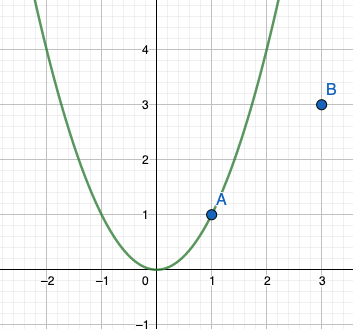
\includegraphics[width=4.5cm, height=4cm]{Esempio-grafico.png}
    \caption{$f(x) = x^2$ con $f: \mathbb{R} \longrightarrow \mathbb{R}$}
    \label{fig:esempio-grafico}
\end{wrapfigure}
\begin{example}
Esempio punto sulla funzione
\begin{itemize}
    \item Il punto A sta sul grafico si $f(x) = x^2$ esattamente quando $y = x^2$.
    \item Il punto B non sta sul grafico quindi $y \neq x^2$.
\end{itemize}
\end{example}
\begin{note}
    A X B $\subseteq \mathbb{R}$ X $\mathbb{R}$. Dove R X R = $R^2$.
\end{note}
\begin{example}
A e B = $(0, +\infty)$, da qui vediamo che A X B rappresenta il primo quadrante.\\\\
\end{example}

\subsection{Immagine}
\begin{definition}[Immagine]
Prendendo $f: A \longrightarrow B$ e $D \subseteq A$ l'immagine di D tramite f è il sottoinsieme $f(D) \subseteq B$ costituito dagli elementi f(d) dove $d \in D$.
\end{definition}
\begin{example}
    Esempi immagine:
    \begin{itemize}
        \item Immagine di A, $f(A) \subseteq B$ si chiama anche immagine della funzione.
        \item $f(x) = x^2$, $f: \mathbb{R} \longrightarrow \mathbb{R}$ \hspace{.2cm} immagine di g è $[0, +\infty)$ perché $x^2 \geq 0 \: \forall \: x \in \mathbb{R}$.
        \item $g(x) = x?2$, $g:[2, +\infty) \longrightarrow \mathbb{R}$ \hspace{.2cm} l'immagine di g è $[4, +\infty]$ perché se si calcola il punto minore del dominio, cioè 2, torna $g(2) = x^2$ che è uguale a 4, da lì possiamo prendere tutti i punti.
    \end{itemize}
\end{example}

\subsection{Suriettiva}
\begin{definition}[Suriettiva]
Una funzione si dice suriettiva quando ogni elemento del codominio è immagine di almeno un elemento del dominio. Quindi prendendo una f(x), per che sia suriettiva deve l'immagine I essere uguale ad un valore, $I(f) = b$.
\end{definition}
\begin{equation}
	\forall y \in B \exists x \in A
\end{equation}
\begin{note}
	La suriettività si traduce graficamente nel fatto una qualsiasi retta orizzontale intersechi il grafico almeno una volta.
\end{note}
\begin{example}
    Esempi funzioni suriettive:
    \begin{itemize}
        \item $f(x) = x^2$, $f: \mathbb{R} \longrightarrow \mathbb{R}$ non è suriettiva perché tutti i valori del codominio $y < 0$ non hanno un rispettivo nel dominio.
        \item $g(x) = x^2$, $g: \mathbb{R} \longrightarrow (0, +\infty)$ lo è perchè andiamo a restringere il codominio ai punti che hanno un corrispettivo nel dominio.
    \end{itemize}
\end{example}

\subsection{Iniettiva}
\begin{definition}[Iniettiva]
Una funzione iniettiva è una funzione che associa, a elementi distinti del dominio, elementi distinti del codominio. Quindi prendendo una f(x) è iniettiva se prendendo due valori $x_1, x_2$ dove $x_1 \neq x_2 \Longrightarrow f(x_1) \neq f(x_2)$. (Input diversi danno output diversi).
\end{definition}
\begin{equation}
	x_{1}, x_{2} \in A \wedge x_{1} \neq x_{2} \implies f(x_{1}) \neq f(x_{2})
\end{equation}
\begin{note}
	L'iniettività si traduce graficamente nel fatto una qualsiasi retta orizzontale intersechi il grafico al più una volta.
\end{note}
\begin{example}
    Esempi funzioni iniettiva:
    \begin{itemize}
        \item $f(x) = x^2$, $f: \mathbb{R} \longrightarrow \mathbb{R}$ non è iniettiva perché se prendiamo $x_1 = 1$ e $x_2 = -1$ $f(x1) = f(x2).$
        \item $g(x) = x^2$, $g: [0, +\infty) \longrightarrow \mathbb{R}$ è invece iniettiva perché non consideriamo i valori negativi.
    \end{itemize}
\end{example}

\subsection{Biunivoca}
\begin{definition}[Biunivoca]
Una funzione si definisce biunivoca o bigettiva se è sia iniettiva che suriettiva.
\end{definition}

\subsection{Invertibile}
\begin{definition}[Invertibile]
Se una funzione è biunivoca si dice che tale funzione è anche invertibile.
\end{definition}
\begin{wrapfigure}{l}{6cm}
    \centering
    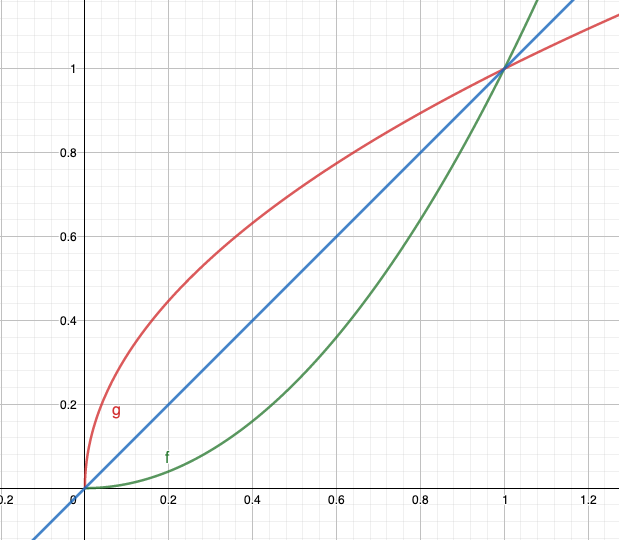
\includegraphics[width=5cm, height=4cm]{Esempio-invertibilita.png}
    \caption{$f(x) = x^2$ e $g(x) = \sqrt{x}$}
    \label{fig:esempio-invertibilità}
\end{wrapfigure}
Se f è una funzione invertibile i grafici di f e di $f^{-1}$ (la funzione inversa) sono simmetrici rispetto alla retta $y=x$ cioè alla bisettrice del primo e del terzo quadrante. \\
\begin{example}
Se vediamo nell'immagine [\ref{fig:esempio-invertibilità}] prendendo l'inverso della funzione $f(x) = x^2$ definita in $[0, +\infty] \longrightarrow \mathbb{R}$ e cioè la funzione $g(x) = \sqrt{x}$ è simmetrica.
\\ \\ \\ \\ \\
\end{example}

\subsection{Funzioni Monotone}
\begin{definition}[Monotone]
Dati $A, B \in \mathbb{R}$ e $f:A \longrightarrow B$. $x_1, x_2 \in A$ con $x_1 < x_2$ se $\forall x_1, x_2$ risulta ciò che è scritto in Tabella \ref{tab:monotone}.
\end{definition}
\begin{table}[h!]
    \centering
    \setlength{\tabcolsep}{6pt}
    \renewcommand{\arraystretch}{1.7}
    \begin{tabular}{|c|c|}
        \hline
        \textbf{[1] Strettamente Crescente} & $f(x_1) < f(x_2) $ \\ \hline
        \textbf{[2]Debolmente Crescente} & $f(x_1) \leq f(x_2) $ \\ \hline
        \textbf{[3]Strettamente Decrescente} & $f(x_1) > f(x_2) $ \\ \hline
        \textbf{[4]Debolmente Decrescente} & $f(x_1) \geq f(x_2) $ \\ \hline
    \end{tabular}
    \caption{Definizioni funzioni crescenti e decrescenti}
    \label{tab:monotone}
\end{table}
Andando a considerare la Tabella \ref{tab:monotone} possiamo dire che:
\begin{itemize}
    \item \textbf{Strettamente monotona} nei casi [1] e [3] della tabella.
    \item \textbf{Debolmente monotona} nei casi [2] e [4] della tabella.
\end{itemize}

\begin{observation}
	Se $f$ è \textbf{strettamente monotona} allora è \textbf{iniettiva} in quanto dati $x_{1} \neq x_{2}$ con $x_{1} < x_{2} \implies f(x_{1}) < f(x_{2})$ e in particolare $f(x_{1}) \neq f(x_{2})$. Non vale però il contrario, infatti una funzione iniettiva non è per forza strettamente monotona (ad esempio data $f(x)=\frac{1}{x}$ con $f:\mathbb{R} \setminus \{0\} \longrightarrow \mathbb{R} \setminus \{0\}$ )
\end{observation}

\begin{observation}
	Se $f$ è \textbf{strettamente crescente} allora è anche \textbf{debolmente crescente}.
\end{observation}
\begin{example}
    Esempi funzioni crescenti e decrescenti:\\
    \begin{figure}[h!]
        \begin{subfigure}{.5\textwidth}
            \centering
            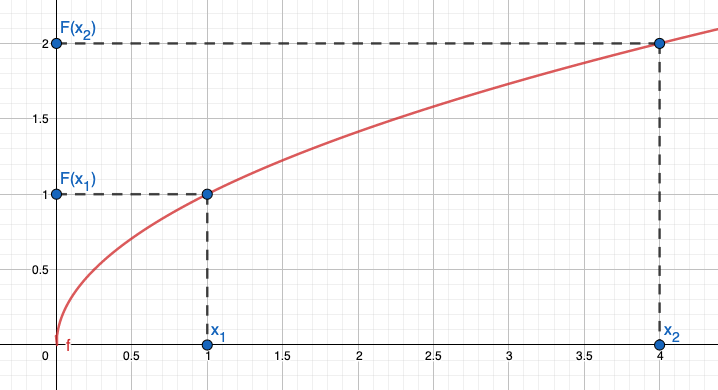
\includegraphics[width=6cm, height=4cm]{funzione-crescente.png}
            \caption{$f(x_1) < f(x-2)$ quindi è crescente}
            \label{fig:funzione-crescente}
        \end{subfigure}
        \begin{subfigure}{.5\textwidth}
            \centering
            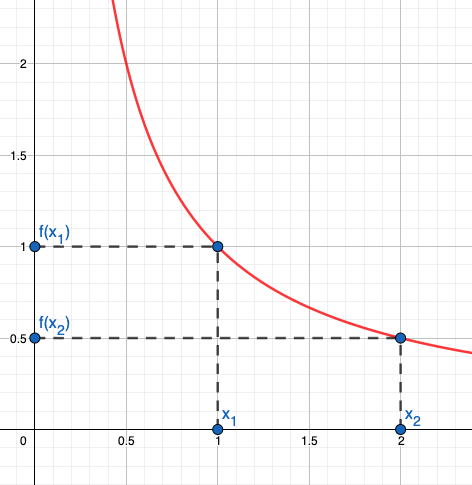
\includegraphics[width=6cm, height=4cm]{funzione-decrescente.png}
            \caption{$f(x_1) > f(x-2)$ quindi è decrescente}
            \label{fig:funzione-decrescente}
        \end{subfigure}
    \end{figure}
    \\Possiamo anche federe dalle immagini [\ref{fig:funzione-crescente}] [\ref{fig:funzione-decrescente}] che:
    \begin{itemize}
        \item Se f(x) è \textbf{crescente} l'ordinamene verrà \textbf{mantenuto}.
        \item Se f(x) è \textbf{decrescente} l'ordinamento verrà \textbf{invertito}.\\
    \end{itemize}
\end{example}

\newpage
\begin{observation}
    Osservazione sul rapporto incrementale:\\
\end{observation}
\begin{wrapfigure}[8]{l}{8cm}
    \vspace{-15pt}
    \centering
    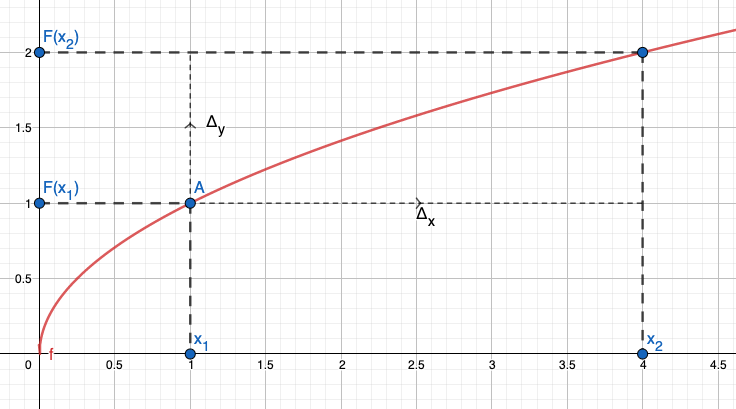
\includegraphics[width=6.7cm]{rapporto_incrementale.png}
    \caption{$\frac{\Delta_y}{\Delta_x}$}
    \label{fig:esempio-invertibilità}
\end{wrapfigure}
Definito il \textbf{rapporto incrementale}\footnote{I rapporto incrementale misura quanto il punto della f si sposta in verticale in rapporto a quanto abbiamo l'asciasse in orizzontale.} come:
\begin{equation}
    \frac{\Delta_y}{\Delta_x}=\frac{f(x_1) - f(x_2)}{x_1 - x_2}
\end{equation}

\begin{note}
    Il denominatore ed il numeratori devono essere concordi per fare in modo che il rapporto incrementale sia maggiore di 0 e quindi la funzione crescente. \\ \\\\
\end{note}
Continuando ad analizzare il rapporto incrementale possiamo ricavare anche i casi in cui una funzione e strettamente decrescente o debolmente crescente o debolmente decrescente. Puoi vedere tutte le casistiche nella tabella \ref{tab:analisi-rapporto-incrementale}.
\begin{table}[h!]
    \centering
    \setlength{\tabcolsep}{7pt}
    \renewcommand{\arraystretch}{2}
    \begin{tabular}{|c|c|}
        \hline
        Strettamente Crescente & $\frac{f(x_1) - f(x_2)}{x_1 - x_2} > 0$\\ \hline
        Strettamente Decrescente & $\frac{f(x_1) - f(x_2)}{x_1 - x_2} < 0$ \\ \hline
        Debolmente Crescente & $\frac{f(x_1) - f(x_2)}{x_1 - x_2} \geq 0$ \\ \hline
        Debolmente Decrescente & $\frac{f(x_1) - f(x_2)}{x_1 - x_2} \leq 0$ \\ \hline
    \end{tabular}
    \caption{Analisi rapporto incrementale}
    \label{tab:analisi-rapporto-incrementale}
\end{table}
\begin{observation}
    Se una funzione f(x) è strettamente crescente è a sua volta anche debolmente crescente, mentre una funzione f(x) se è debolmente crescente non è strettamente crescente perché aggiunge una casistica che sarebbe $f(x_1) = f(x_2)$. 
\end{observation}
\begin{example}
    Casistica particolare:\\
    Data $f(x)=\frac{1}{x}$, \hspace{.3cm} $f: \mathbb{R} \: \setminus \: \{0\} \longrightarrow \mathbb{R} \: \setminus \: \{0\}$. Funzione rappresentata nell'immagine [\ref{fig:esempio-particolare}].
    \begin{figure}[h!]
        \centering
        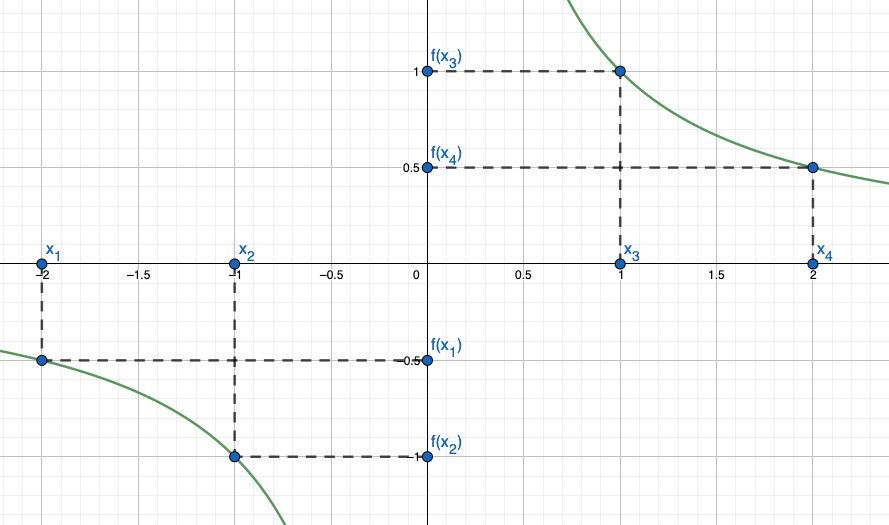
\includegraphics[width=8.7cm]{esempio-particolare.png}
        \caption{$f(x)=\frac{1}{x}$, \hspace{.3cm} $f: \mathbb{R} \: \setminus \: \{0\} \longrightarrow \mathbb{R} \: \setminus \: \{0\}$}
        \label{fig:esempio-particolare}
    \end{figure}
    \\Possiamo vedere che:
    \begin{itemize}
        \item f(x) è strettamente decrescente in $(0, +\infty)$.\\
        Quindi se andiamo a prendere $0 < x_3 < x_4$ abbiamo che $f(x_3) > f(x_4)$.
        \item f(x) è strettamente decrescente in $(-\infty, 0)$.\\
        Quindi se andiamo a prendere $x_1 < x_2 < 0$ abbiamo che $f(x_1) > f(x_2)$.
    \end{itemize}
    Se però andiamo a considerare tutto $\mathbb{R} \: \setminus \: \{0\}$, e quindi prendiamo i punti $x_1 < 0 < x_4$ vediamo che $f(x_1) < f(x_4)$.
    In conclusione si può dire quindi che $f(x)=\frac{1}{x}$) è decrescente in $(-\infty, 0)$ e in $(0, +\infty)$ ma non lo è in tutto $\mathbb{R} \: \setminus \: \{0\}$.
\end{example}

\subsubsection{Composizione con funzioni monotone}
\begin{definition}[Composizione]
	La composizione di funzioni si definisce come $g \circ f:A \longrightarrow C$, $(g \circ f)(a)=g(f(a))$
\end{definition}
Prendendo i considerazioni 3 insiemi A, B, C tali che $A, B, C \subset \mathbb{R}$ e 2 funzioni f(x) e g(x) così definite: \hspace{.2cm} $f: A \longrightarrow B$, $g: B \longrightarrow C $.
\begin{enumerate}
    \item Se f è crescente e g è crescente allora $g \circ f$ è crescente.
    \item Se f è crescente e g è decrescente allora $g \circ f$ è decrescente e viceversa ($ x_{1} < x_{2} \implies f(x_{1}) < f(x_{2}) \implies g(f(x_{1})) < g(f(x_{2})) $).
    \item Se f è decrescente e g è decrescente allora $g \circ f$ è crescente ($ x_{1} < x_{2} \implies f(x_{1}) > f(x_{2}) \implies g(f(x_{1})) < g(f(x_{2})) $).
\end{enumerate}

\begin{example}
    $h(x) = e^{x^3}$\\
    La funzione $h$ si ottiene dalla composizione di:
    \begin{itemize}
        \item $f: \mathbb{R} \longrightarrow \mathbb{R}$ \hspace{.3cm} $f(x) = x^3$. Funzione crescente.
        \item $g: \mathbb{R} \longrightarrow \mathbb{R}$ \hspace{.3cm} $g(t) = e^t$. Funzione decrescente.
    \end{itemize}
    Quindi possiamo scrivere $h(x) = e^{x^3}$ come: \hspace{.3cm} $e^{f(x)} \: \: = \: \: g(f(x)) \: \: = \: \: (g \circ f)(x)$
    Inoltre visto che f è crescente e g è crescente, h è strettamente crescente 
\end{example}
\begin{observation}
    Se prendiamo una funzione f(x) strettamente monotona, allora f(x) è iniettiva. Questa condizione è vera ma NON lo è viceversa: una funzione f(x) iniettiva NON è per forza strettamente monotona. 
\end{observation}
\begin{example}
    Se prendiamo una f(x) tale che: \hspace{.3cm} $f(x) = \frac{1}{x}$ \hspace{.3cm} $\mathbb{R} \setminus \{0\} \longrightarrow \mathbb{R} \setminus \{0\}$
    \\Possiamo vedere rifacendoci all'esempio in figura [\ref{fig:esempio-particolare}] che f è iniettiva ma non monotona.
\end{example}

\subsection{Insieme di definizione}
\begin{definition}[Insieme di definizione]
    Data una funzione f(x) l'insieme di definizione o dominio naturale di una funzione è il più grande sottoinsieme di $\mathbb{R}$ dove ha senso la funzione f(x).
\end{definition}
\begin{example}
    $f(x) = \frac{1}{x}$ \hspace{.3cm} L'insieme di definizione è $\mathbb{R} \setminus \{0\}$
\end{example}

\subsection{Funzioni pari e dispari}
\begin{definition}[Pari]
    La funzione è \textbf{pari} se $f(x) = f(-x) \: \forall x$ nel dominio di $f \longrightarrow f$. Il grafico di una funzione pari è simmetrico rispetto all'asse $y$.
\end{definition}
\begin{definition}[Dispari]
    La funzione è \textbf{dispari} se $f(x) = -f(-x) \: \forall x$ nel dominio di $f \longrightarrow f$. Il grafico di una funzione dispari è simmetrico rispetto all'origine.
\end{definition}
\begin{note}
    Il dominio di $f$ deve essere simmetrico.\\
\end{note}
\begin{example}
Esempio funzioni pari e dispari.\\
\end{example}
$f(-x) = (-x)^2 = x^2 = f(x)$, f(x) è \textbf{pari}: \hfill $f(-x) = (-x)^2 = x^2 = -f(x)$, f(x) è \textbf{dispari}:
\begin{figure}[h!]
    \vspace{-1pt}
    \begin{subfigure}{.5\textwidth}
        \centering
        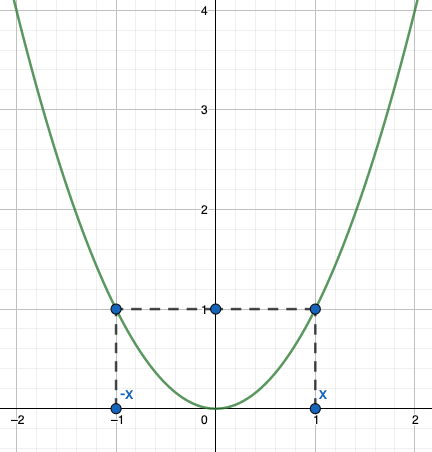
\includegraphics[width=3cm]{funzione-pari.png}
        \caption{$f(x) = x^2$, \hspace{.2cm} graph(f) con f pari}
    \end{subfigure}
    \begin{subfigure}{.5\textwidth}
        \centering
        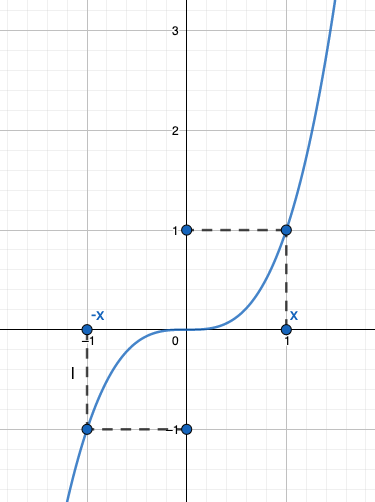
\includegraphics[width=2.5cm]{funzione-dispari.png}
        \caption{$f(x) = x^3$, \hspace{.2cm} graph(f) con f dispari}
    \end{subfigure}
\end{figure}
\begin{note}
	Una funzione del tipo $f(x)=x^(2n)$ con $n \in \mathbb{N}$ è sempre pari mentre una funzione del tipo $f(x)=x^(2n+1)$ con $n \in \mathbb{N}$ è sempre dispari.
\end{note}

\subsection{Funzione periodica}
\begin{definition}[Periodicità]
    Una funzione f(x) si dice periodica di periodo $P \in \mathbb{R}$ se $\forall x \: \: f(x + P) = f(x)$. 
\end{definition}
\begin{wrapfigure}{r}{9cm}
    \vspace{-15pt}
    \centering
    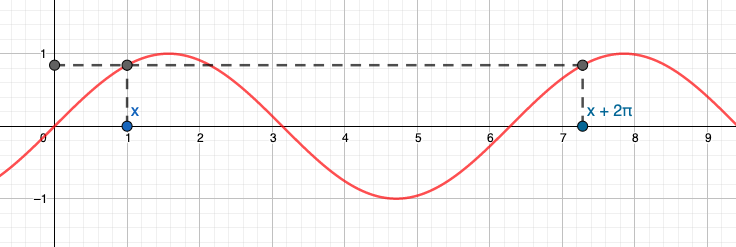
\includegraphics[width=7cm]{funzione-periodica.png}
    \caption{$sin(x) = sin(x + 2\pi)$}
    \label{fig:funzione-periodica}
\end{wrapfigure}
Inoltre il dominio di f(x) deve essere tale che $x \in dom(f) \implies x + P \in dom(f)$.
\begin{example}
In figura [\ref{fig:funzione-periodica}] un esempio di funzione periodica.\\\\
\end{example}

\subsection{Funzioni Elementari}
\subsubsection{Lineari}
\textbf{Funzione retta}: $f(x) = ax + b$. \hspace{.3cm} $a,b \in \mathbb{R}$ \\ Dove $a$ (coefficiente angolare) indica la pendenza della retta, mentre $b$ (termine noto) indica il punto di incontro con l'asse $Y$.

\subsubsection{Esponente positivo o negativo}
\textbf{Fun. Esp. positivo:} $f(x) = x^k$, $k \in \mathbb{N}$. \hfill \textbf{Fun. Esp. negativo:} $f(x) = x^k$, $k \in \mathbb{N}$, $k < 0$.
\begin{figure}[h!]
    \begin{subfigure}{.5\textwidth}
        \centering
        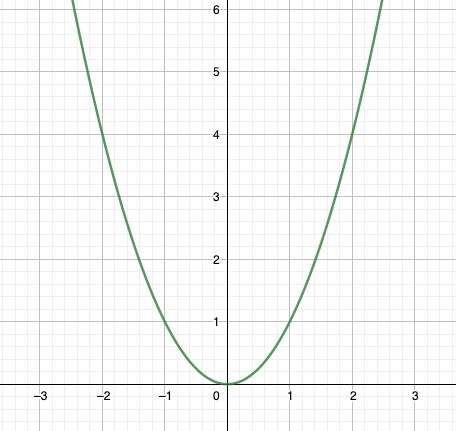
\includegraphics[width=4cm, height=3.5cm]{parabole.png}
        \caption{con k pari}
        \label{fig:esponente-positivo-pari}
    \end{subfigure}
    \begin{subfigure}{.5\textwidth}
        \centering
        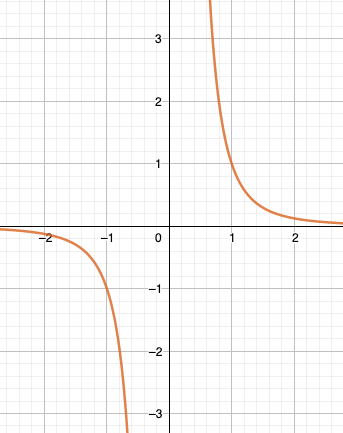
\includegraphics[width=4cm, height=3.5cm]{esponente-negativo-dispari.png}
        \caption{con k dispari}
        \label{fig:esponente-positivo-dispari}
    \end{subfigure}
\end{figure}
\begin{figure}[h!]
    \vspace{-5pt}
    \begin{subfigure}{.5\textwidth}
        \centering
        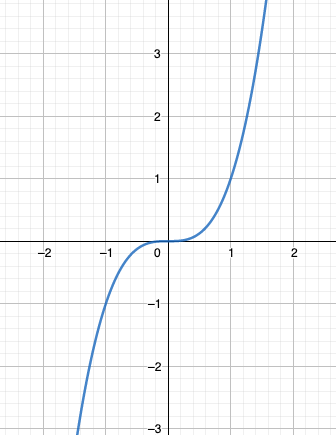
\includegraphics[width=4cm, height=3.7cm]{esponente-dispari.png}
        \caption{con k pari}
        \label{fig:esponente-negativo-pari}
    \end{subfigure}
    \begin{subfigure}{.5\textwidth}
        \centering
        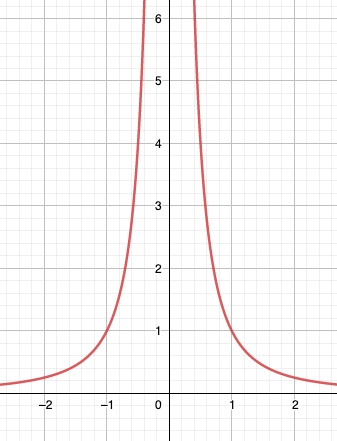
\includegraphics[width=4cm, height=3.5cm]{esponsente-negativo-pari.png}
        \caption{con k dispari}
        \label{fig:esponente-negativo-dispari}
    \end{subfigure}
\end{figure}
\begin{observation}
    \textbf{k pari}: Le funzioni con il $k$ pari sono funzioni pari e hanno tutte una forma simile a quella in figura [\ref{fig:esponente-positivo-pari}] per le funzioni con k positive e per le funzioni con k negativo figura [\ref{fig:esponente-negativo-pari}].
\end{observation}
\begin{observation}
    \textbf{k dispari:} Le funzioni con il k positivo e dispari sono funzioni dispari e hanno tutte una forma simile a quella in figura [\ref{fig:esponente-positivo-dispari}] per le funzioni con k positive e per le funzioni con k negativo figura [\ref{fig:esponente-negativo-dispari}].
\end{observation}

\subsubsection{Radici o esponente fratto}
\textbf{Funzionane radici o esponente fratto:} $f(x) = x^{\frac{p}{q}}$ o $f(x) = \sqrt[q]{x^p}$  \: \: con  \: \:  $p, q \in \mathbb{N}$ \: \: e  \: \:  $q \neq 0$. \footnote{In matematica è possibile scrivere una un esponente fratto come radice mettendo il numeratore al radicando della radice e il denominatore all'indice: $x^{\frac{p}{q}} \: = \: \sqrt[q]{x^p}$}
\begin{figure}[h!]
    \begin{subfigure}{.5\textwidth}
        \centering
        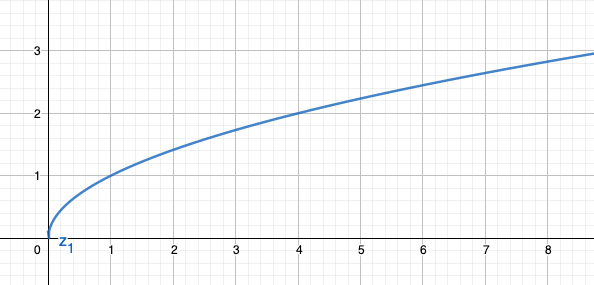
\includegraphics[width=6.3cm]{radice-pari.png}
        \caption{con q pari}
        \label{fig:radice-pari}
    \end{subfigure}
    \begin{subfigure}{.5\textwidth}
        \centering
        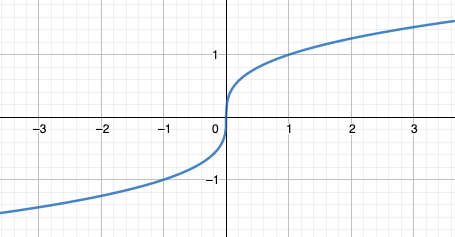
\includegraphics[width=6cm]{radice-dispari.png}
        \caption{con q dispari}
        \label{fig:radice-dispari}
    \end{subfigure}
\end{figure}
\begin{note}
    $p$ e $q$ non possono essere entrambi pari perché in tal caso sono divisibili fra di loro e quindi portabili ad una forma ridotta.
\end{note}
\begin{observation}
    \textbf{q pari:} Le funzioni con il $q$ pari ha dominio $ x \geq 0$ ed è invertibile sono come funzione $f: [0, +\infty) \longrightarrow [0, +\infty)$. È rappresentata in figura [\ref{fig:radice-pari}].
\end{observation}
\begin{observation}
    \textbf{q dispari:} Le funzioni con il $q$ positivo ha dominio $x \in \mathbb{R}$ ed è ugualmente invertibile su tutto $\mathbb{R}$, è inoltre una funzione dispari. È rappresentata in figura [\ref{fig:radice-dispari}].\\
\end{observation}

\subsubsection{Esponenziale}
\textbf{Funzione esponenziale:} $f(x) = a^x$ con $a \in \mathbb{R}$, \: \: $a > 0$, \: \: $a \neq 1$ \: \: $f: \mathbb{R} \longrightarrow (0, +\infty)$
\begin{figure}[h!]
    \begin{subfigure}{.5\textwidth}
        \centering
        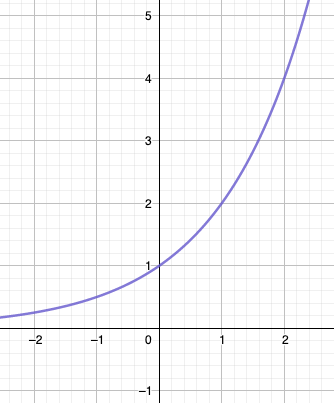
\includegraphics[width=4cm]{esponenziale.png}
        \caption{con $a > 1$}
        \label{fig:esponenziale}
    \end{subfigure}
    \begin{subfigure}{.5\textwidth}
        \centering
        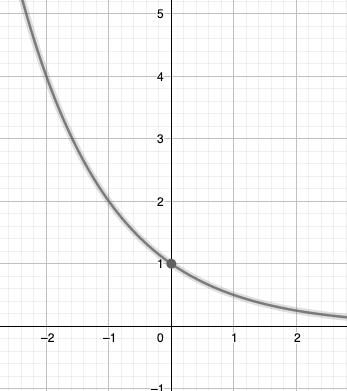
\includegraphics[width=4cm]{esponsenziale-base-minore.png}
        \caption{con $0 < a < 1$}
        \label{fig:esponsenziale-base-minore}
    \end{subfigure}
\end{figure}
\begin{note}
    La funzione esponenziale è sempre positiva.
\end{note}
\begin{observation}
    \textbf{$a > 1$:} La funzione è strettamente crescente, come in nell'immagine [\ref{fig:esponenziale}].
\end{observation}
\begin{observation}
    \textbf{$0 < a < 1$:} La funzione è decrescente, come in nell'immagine [\ref{fig:esponsenziale-base-minore}].
\end{observation}

\subsubsection{Logaritmo}
\textbf{Funzione logaritmo:} $f(x) = \log_a x$, \: \: $f: (0, +\infty) \longrightarrow \mathbb{R}$ \: \: (inversa dell'esponenziale).
\begin{figure}[h!]
    \begin{subfigure}{.5\textwidth}
        \centering
        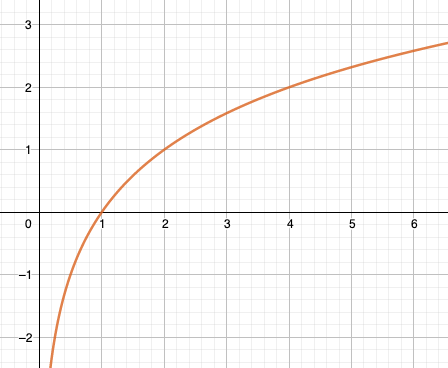
\includegraphics[width=5cm,height=4cm]{logaritmo.png}
        \caption{con $a > 1$}
        \label{fig:logaritmo}
    \end{subfigure}
    \begin{subfigure}{.5\textwidth}
        \centering
        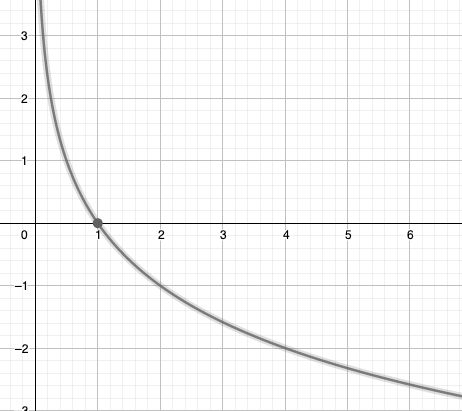
\includegraphics[width=5cm,height=4cm]{logaritmo-base-minore.png}
        \caption{con $0 < a < 1$}
        \label{fig:logaritmo-base-minore}
    \end{subfigure}
\end{figure}
\begin{observation}
    Casistica particolare - $f(x) = e^x$.\\
    In questa casistica se andiamo a ridurre il codominio la funzione esponenziale è invertibile. $f: \mathbb{R} \longrightarrow (0, +\infty)$.
    Il suo inverso è un caso particolare di logaritmo e di chiama \textbf{logaritmo naturale}. E si può scrive in due modi:
    \begin{itemize}
        \item $\ln{x}$: sarebbe logaritmo in base naturale.
        \item $\log x$: scrivendo il logaritmo senza la base intendiamo il logaritmo in base $e$.
    \end{itemize}
\end{observation}

\subsubsection{Seno e Arcoseno}
\textbf{Seno:} $f(x) = \sin x$, $f: \mathbb{R} \longrightarrow \mathbb{R}$. \hfill
\textbf{Arcoseno:} $f(x) = \arcsin x$, $f: [-1, 1] \longrightarrow [-\frac{\pi}{2}, \frac{\pi}{2}]$
\begin{figure}[h!]
    \begin{subfigure}{.5\textwidth}
        \centering
        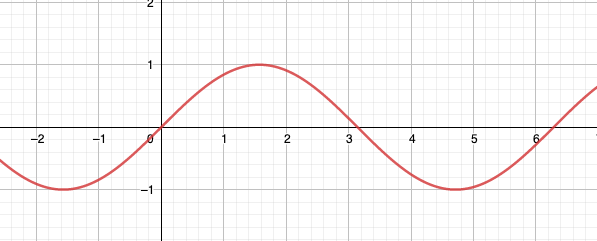
\includegraphics[width=6cm]{seno.png}
        \caption{$\sin{x}$}
        \label{fig:seno}
    \end{subfigure}
    \begin{subfigure}{.5\textwidth}
        \centering
        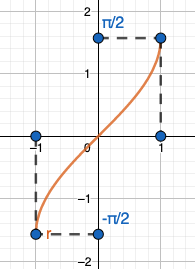
\includegraphics[width=2cm, height=2.3cm]{arcoseno.png}
        \caption{$\arcsin{x}$ o $\sin{x}^{-1}$}
        \label{fig:arcoseno}
    \end{subfigure}
\end{figure}

\begin{observation}
    \textbf{Sin(x):} La funzione $\sin{x}$ (immagine [\ref{fig:seno}]) è periodica per $2\pi$ quindi possiamo scrivere $\sin{(x+2\pi)} = \sin x \: \forall x \in \mathbb{R}$. Inoltre è suriettiva per codominio [-1, 1]. Se invece definiamo $f: [-\frac{\pi}{2}, \frac{\pi}{2}] \longrightarrow [-1, 1]$ la funzione $\sin x$ è strettamente crescente e suriettiva, quindi anche invertibile, e la sua inversa è appunto $\arcsin{x}$.
\end{observation}
\begin{observation}
    \textbf{Arcsin(x):} La funzione $\arcsin{x}$ è l'inverso del seno e può essere scritta anche come $f(x) = \sin{x}^{-1}$, è rappresentata nell'immagine [\ref{fig:arcoseno}].
\end{observation}

\subsubsection{Coseno e Arcocoseno}
\textbf{Coseno:} $f(x) = \cos{x}$, $f: \mathbb{R} \longrightarrow \mathbb{R}$. \hfill
\textbf{Arcocoseno:} $f(x) =\arccos{x}$, $f: [-1, 1] \longrightarrow [0, \pi]$
\begin{figure}[h!]
    \begin{subfigure}{.5\textwidth}
        \centering
        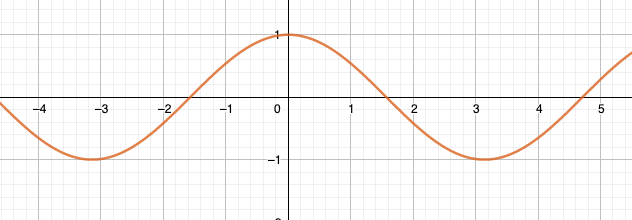
\includegraphics[width=6cm]{coseno.png}
        \caption{$\cos{x}$}
        \label{fig:coseno}
    \end{subfigure}
    \begin{subfigure}{.5\textwidth}
        \centering
        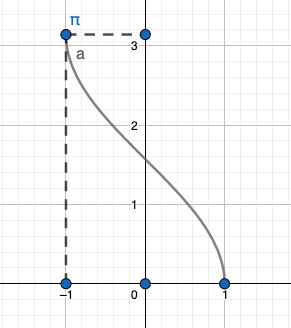
\includegraphics[width=3.5cm, height=2.7cm]{arcocoseno.png}
        \caption{$\arccos{x}$ o $\cos{x}^{-1}$}
        \label{fig:arcocoseno}
    \end{subfigure}
\end{figure}
\vspace{-5pt}
\begin{observation}
    \textbf{Cos(x):} La funzione $\cos{x}$, rappresentata nell'immagine [\ref{fig:coseno}], è periodica per $2\pi$ quindi possiamo scrivere $\cos{(x+2\pi)} = \cos x \: \forall x \in \mathbb{R}$. Inoltre è suriettiva per codominio [-1, 1]. Se invece definiamo $f: [0, \pi] \longrightarrow [-1, 1]$ la funzione $\cos x$ è suriettiva, quindi anche invertibile, e la sua inversa è appunto $\arccos{x}$.
\end{observation}
\begin{observation}
    \textbf{Arccos(x):} La funzione $\arccos{x}$ è l'inverso del seno e può essere scritta anche come $f(x) = \cos{x}^{-1}$ ed è rappresentata nell'immagine [\ref{fig:arcocoseno}].
\end{observation}

\subsubsection{Tangente e Arcotangente}
\textbf{Tangente:} $f(x) = \tan{x}$, $f: \mathbb{R} \longrightarrow \mathbb{R}$ \hfill
\textbf{Arcotangente:} $f(x) = \arctan{x}$, $f: \mathbb{R} \longrightarrow [-\frac{\pi}{2}, \frac{\pi}{2}]$
\begin{figure}[h!]
    \begin{subfigure}{.5\textwidth}
        \vspace{-20pt}
        \centering
        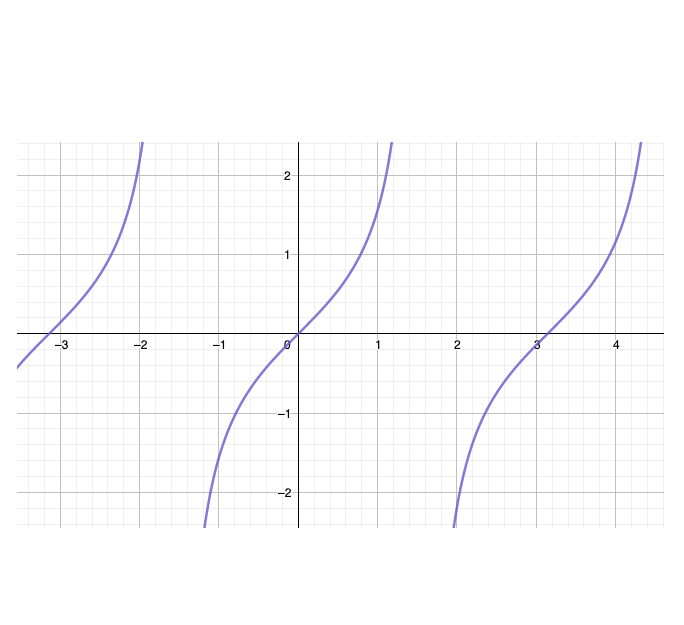
\includegraphics[width=4.2cm]{tangente.png}
        \vspace{-20pt}
        \caption{$\tan{x}$}
        \label{fig:tangente}
    \end{subfigure}
    \begin{subfigure}{.5\textwidth}
        \centering
        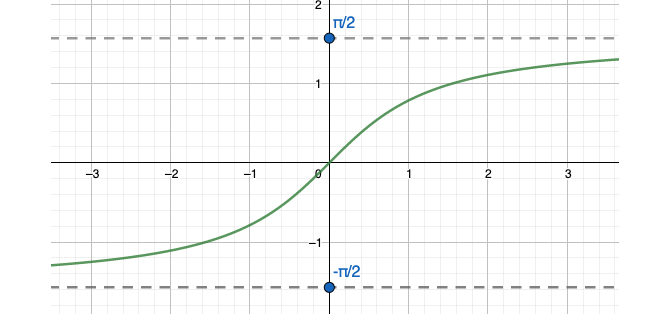
\includegraphics[width=5cm]{arcotangente.png}
        \caption{$\arctan{x}$ o $\tan{x}^{-1}$}
        \label{fig:arcotangente}
    \end{subfigure}
\end{figure}
\begin{observation}
    \textbf{Tan(x):} La funzione $\tan{x}$, rappresentata nell'immagine [\ref{fig:tangente}], può essere scritta anche come $\frac{\sin{x}}{\cos{x}}$, ha come dominio $\{x \in \mathbb{R} \: | \:  x \neq \frac{\pi}{2} + k\pi, \: k \in \mathbb{Z}\}$. La funzione tangente è fatta da infiniti intervalli, è quindi periodica per $\pi$; è di base non invertibile, ma se la ristringiamo in $f: [-\frac{\pi}{2}, \frac{\pi}{2}] \longrightarrow \mathbb{R}$ diventa biunivoca ed accetta la funzione inversa che è $\arctan{x}$.
\end{observation}
\begin{observation}
    \textbf{Arctan(x):} La funzione $\arctan{x}$, rappresentate nell'immagine [\ref{fig:arcotangente}], è inversa della funzione $\tan{x}$, può quindi essere scritta anche con la forma $\tan{x}^{-1}$.
\end{observation}